\documentclass{../../slides-style}

\slidetitleext{Лекция 8/Практика 7: Поведенческие шаблоны}{15.05.2025}{Поведенческие шаблоны}

\begin{document}

    \begin{frame}[plain]
        \titlepage
    \end{frame}

    \section{Паттерн \enquote{Команда}}

    \begin{frame}{Паттерн \enquote{Команда}, мотивация}
        \begin{outline}
            \1 Хотим отделить инициацию запроса от его исполнения
            \1 Хотим, чтобы тот, кто \enquote{активирует} запрос, не знал, как он исполняется
            \1 При этом хотим, чтобы тот, кто знает, когда исполнится запрос, не знал, когда он будет активирован
            \1 Но зачем?
                \2 Команды меню приложения
                \2 Палитры инструментов
                \2 ...
            \1 \enquote{Просто вызвать действие} не получится, вызов функции жёстко свяжет инициатора и исполнителя
        \end{outline}
    \end{frame}

    \begin{frame}{Решение: обернём действие в объект}
        \begin{center}
            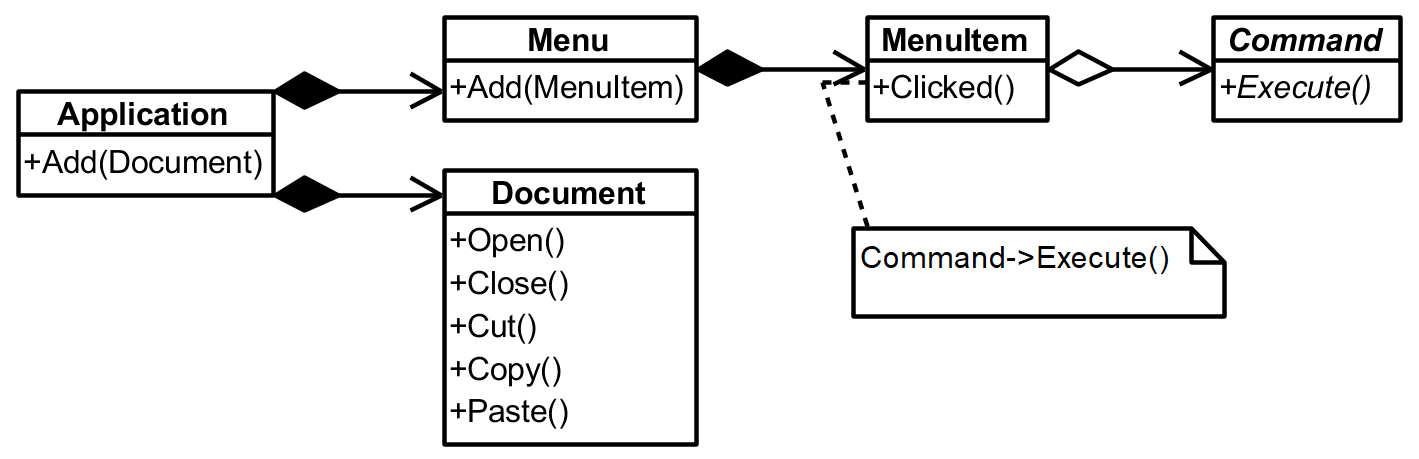
\includegraphics[width=0.9\textwidth]{commandExample.png}
        \end{center}
    \end{frame}

    \begin{frame}{Команда вставки}
        \begin{center}
            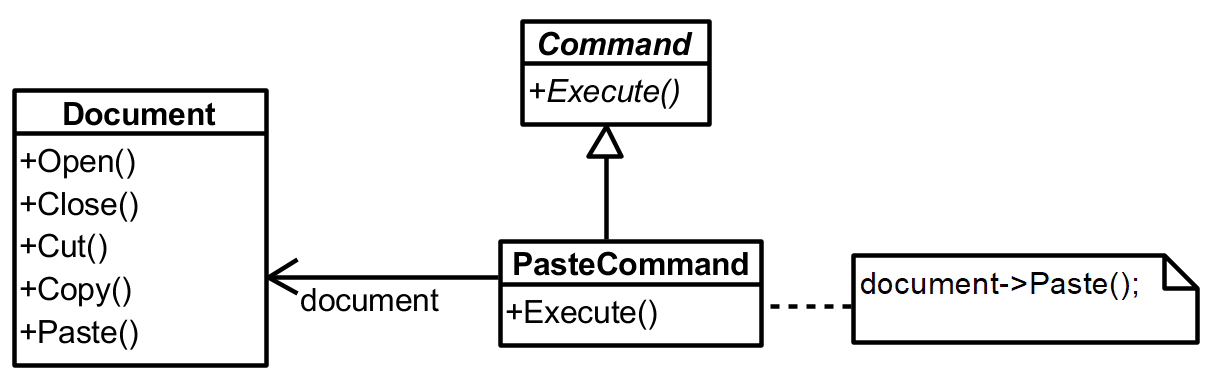
\includegraphics[width=0.75\textwidth]{pasteCommand.png}
        \end{center}
    \end{frame}

    \begin{frame}{Команда открытия документа}
        \begin{center}
            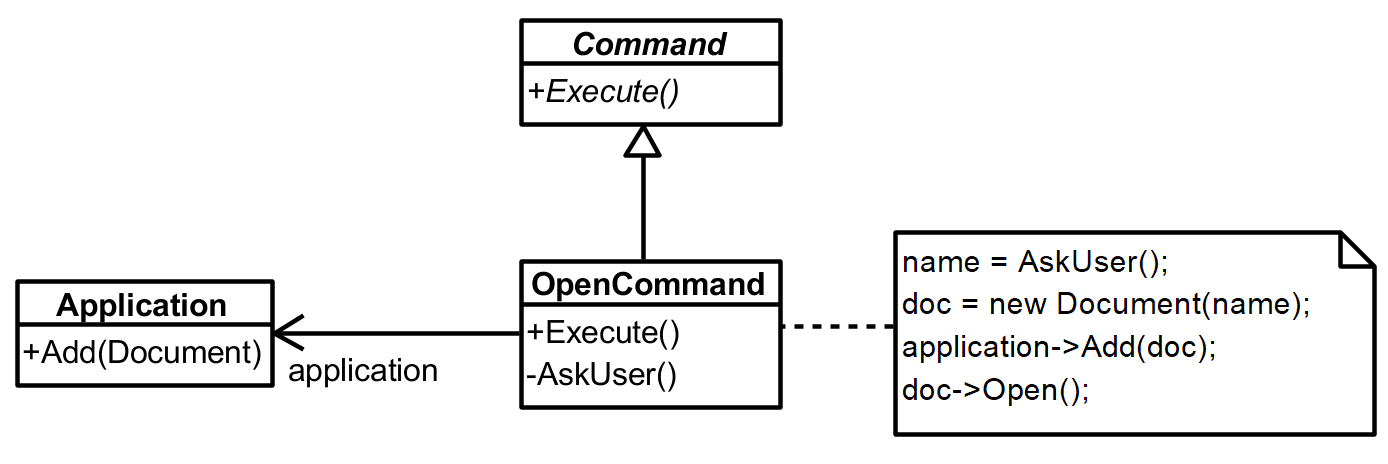
\includegraphics[width=0.75\textwidth]{openDocumentCommand.png}
        \end{center}
    \end{frame}

    \begin{frame}{Составная команда}
        \begin{center}
            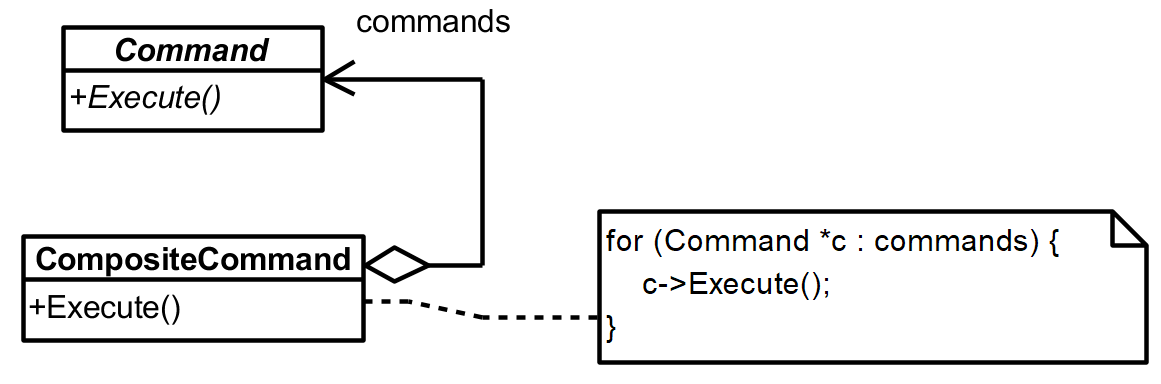
\includegraphics[width=0.75\textwidth]{compositeCommand.png}
        \end{center}
    \end{frame}

    \begin{frame}{Паттерн \enquote{Команда}}
        \begin{center}
            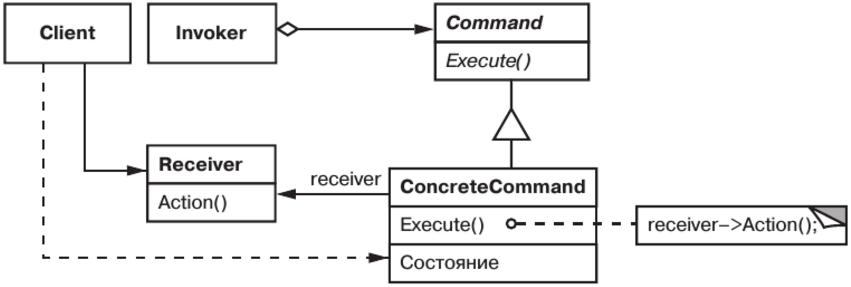
\includegraphics[width=0.9\textwidth]{command.png}
        \end{center}
    \end{frame}

    \begin{frame}{Взаимодействие объектов}
        \begin{center}
            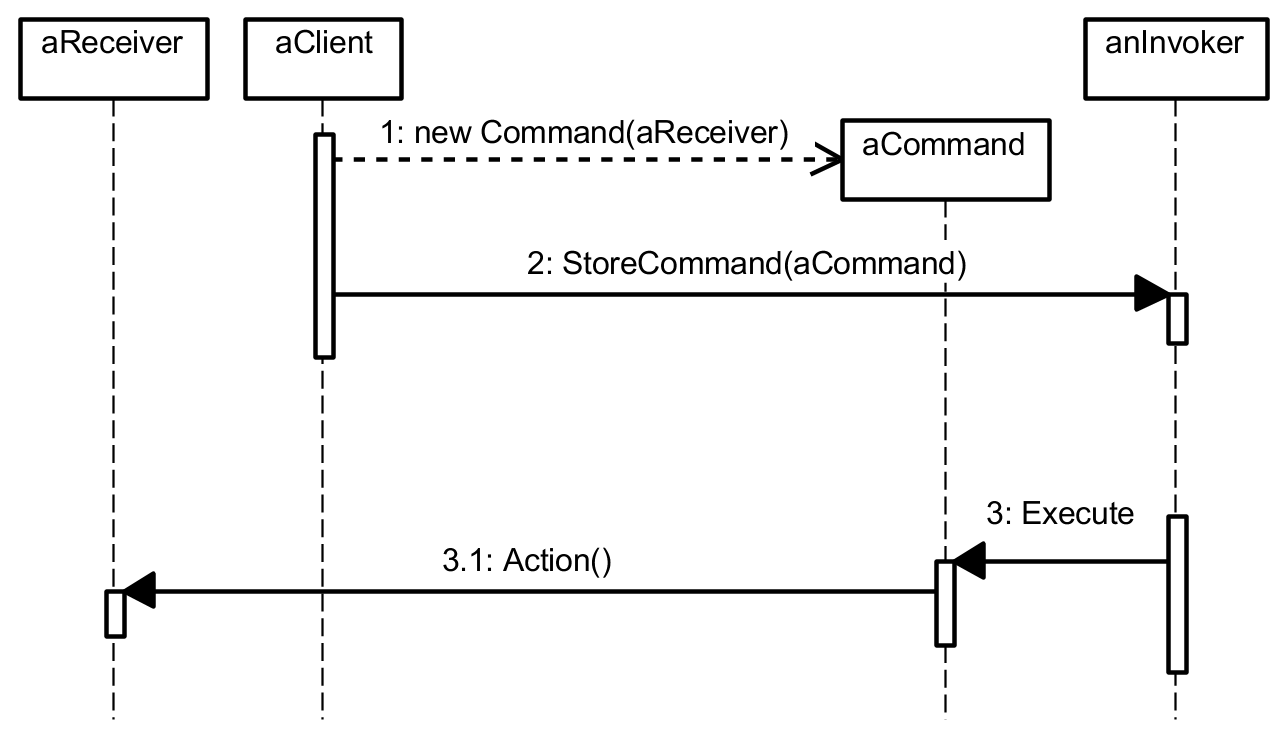
\includegraphics[width=0.9\textwidth]{commandSequence.png}
        \end{center}
    \end{frame}

    \begin{frame}{Команда, применимость}
        \begin{outline}
            \1 Параметризовать объекты выполняемым действием
            \1 Определять, ставить в очередь и выполнять запросы в разное время
            \1 Поддержать отмену операций
            \1 Структурировать систему на основе высокоуровневых операций, построенных из примитивных
            \1 Поддержать протоколирование изменений
        \end{outline}
    \end{frame}

    \begin{frame}{\enquote{Команда} (Command), детали реализации}
        \begin{outline}
            \1 Насколько \enquote{умной} должна быть команда
            \1 Отмена и повторение операций --- тоже от хранения всего состояния в команде до \enquote{вычислимого} отката
                \2 Undo-стек и Redo-стек
                \2 Может потребоваться копировать команды
                \2 \enquote{Искусственные} команды
                \2 Композитные команды
            \1 Паттерн \enquote{Хранитель} для избежания ошибок восстановления
        \end{outline}
    \end{frame}

    \begin{frame}[fragile]{\enquote{Команда}, пример}
        \begin{outline}
            \1 Qt, класс QAction:
            \begin{minted}{c++}
const QIcon openIcon = QIcon(":/images/open.png");
QAction *openAct = new QAction(openIcon, tr("&Open..."), this);

openAct->setShortcuts(QKeySequence::Open);
openAct->setStatusTip(tr("Open an existing file"));

connect(openAct, &QAction::triggered, this, &MainWindow::open);

fileMenu->addAction(openAct);
fileToolBar->addAction(openAct);
            \end{minted}
        \end{outline}
    \end{frame}

    \section{Паттерн \enquote{Хранитель}}

    \begin{frame}{Паттерн \enquote{Хранитель}, мотивация}
        \begin{center}
            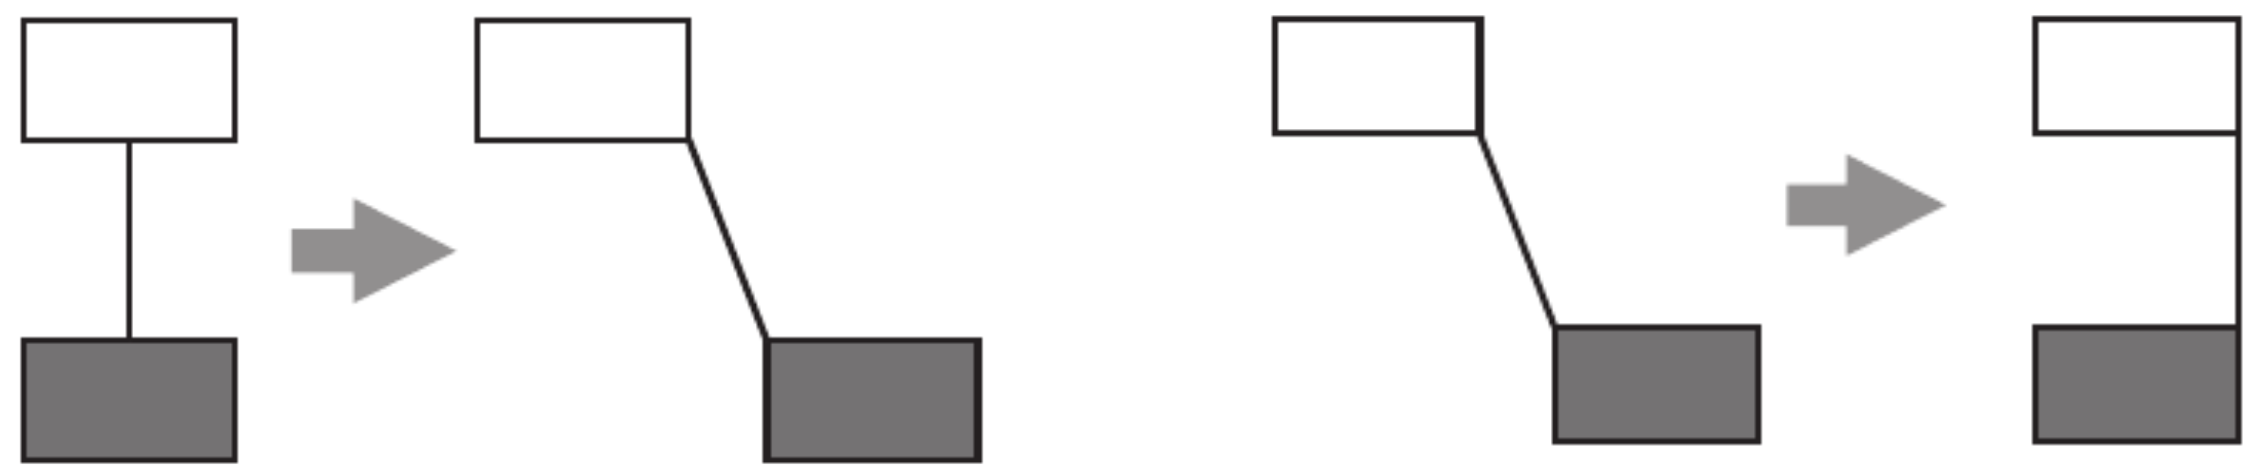
\includegraphics[width=0.9\textwidth]{mementoMotivation.png}
        \end{center}
        \begin{outline}
            \1 Хотим уметь фиксировать внутреннее состояние объектов
            \1 И восстанавливать его при необходимости
            \1 Не раскрывая внутреннего устройства объектов кому не надо
        \end{outline}
    \end{frame}

    \begin{frame}{Паттерн \enquote{Хранитель}}
        \begin{center}
            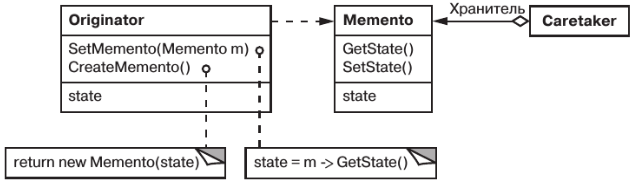
\includegraphics[width=0.7\textwidth]{memento.png}
        \end{center}
    \end{frame}

    \begin{frame}{\enquote{Хранитель} (Memento), детали реализации}
        \begin{outline}
            \1 Два интерфейса: \enquote{широкий} для хозяев и \enquote{узкий} для остальных объектов
                \2 Требуется языковая поддержка
            \1 Можно хранить только дельты состояний
        \end{outline}
    \end{frame}

    \section{Паттерн \enquote{Состояние}}

    \begin{frame}{Паттерн \enquote{Состояние}, мотивация}
        \begin{center}
            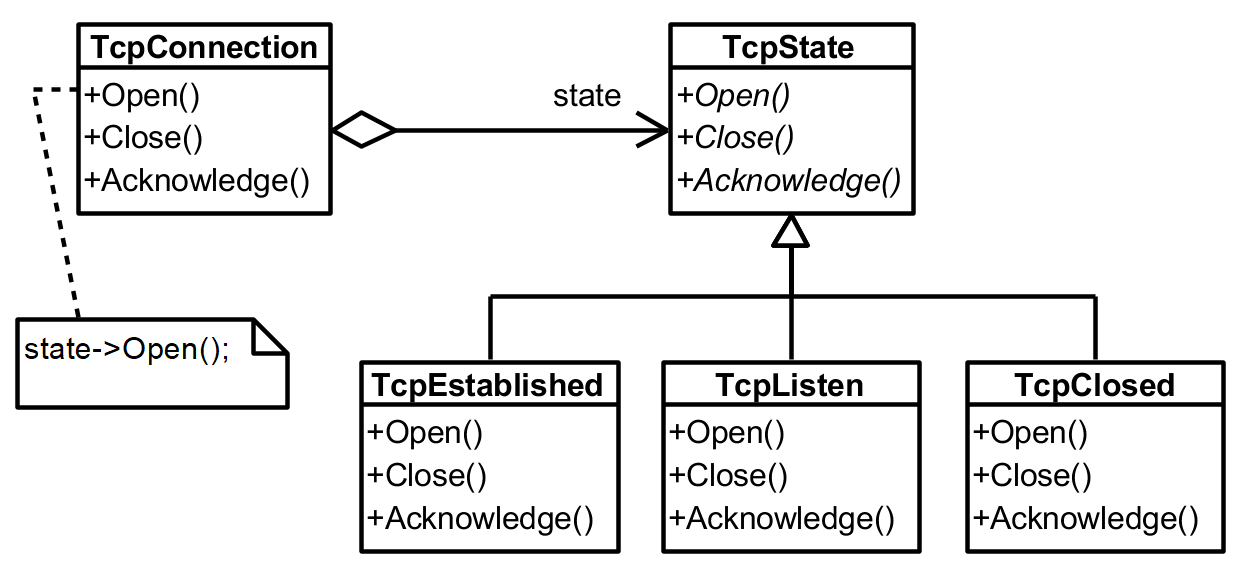
\includegraphics[width=0.85\textwidth]{stateExample.png}
        \end{center}
    \end{frame}

    \begin{frame}{Паттерн \enquote{Состояние}}
        \begin{center}
            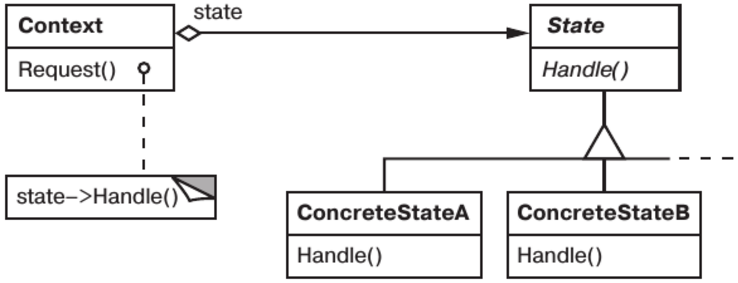
\includegraphics[width=0.75\textwidth]{state.png}
        \end{center}
    \end{frame}

    \begin{frame}{\enquote{Состояние} (State), детали реализации}
        \begin{outline}
            \1 Переходы между состояниями --- в Context или в State?
            \1 Таблица переходов
                \2 Трудно добавить действия по переходу
            \1 Создание и уничтожение состояний
                \2 Создать раз и навсегда
                \2 Создавать и удалять при переходах
        \end{outline}
    \end{frame}

    \begin{frame}{\enquote{Состояние} результаты}
        \begin{outline}
            \1 Локализует зависящее от состояния поведение
            \1 Делает явными переходы между состояниями
            \1 Объекты состояния можно разделять
        \end{outline}
        Когда применять:
        \begin{outline}
            \1 Поведение объекта зависит от его состояния и должно изменяться во время выполнения
            \1 Обилие условных операторов, в которых выбор ветви зависит от состояния
        \end{outline}
    \end{frame}

    \section{Задача}

    \begin{frame}{Задача на дом}
        Уточнить модель компьютерной игры Roguelike:

        \begin{enumerate}
            \item Используя шаблон \enquote{Команда} для поддержки взаимодействия с пользователем
            \item Используя паттерн \enquote{Хранитель} для поддержки сохранения/загрузки игры
            \item Используя паттерн \enquote{Состояние} для динамического переключения поведения мобов
            \begin{outline}
                \1 Мобы с низким здоровьем должны переключаться в трусливый режим
                \1 По мере восстановления здоровья переходить в исходный
            \end{outline}
        \end{enumerate}
    \end{frame}

\end{document}
